%----------------------------------------------------------------------
\section{Success Stories}
\begin{frame}[c]{Success Stories}
\framesubtitle{Spearmint}

\small
\begin{itemize}
    \item First successful open source Bayesian optimization implementation.
    \item Was used to tune a neural network to state-of-the-art performance on CIFAR-10 in 2012.
    \item Implements standard Bayesian optimization with MCMC integration of the acquisition function, asynchronous parallelism, input warping and constraints.
    \item Startup based on Spearmint got acquired by Twitter in 2015.
    \item Still heavily used and cited and available at \url{https://github.com/HIPS/spearmint}:
    \begin{center}
        \only{
\includegraphics[width=0.7\linewidth, keepaspectratio=true]{w07_hpo_grey_box/images/success_stories/jsnoek_spearmint_git_stats.png}}
        
        \only{
\includegraphics[width=0.7\linewidth, keepaspectratio=true]{w07_hpo_grey_box/images/success_stories/hips_spearmint_git_stats.png}}
        
        \only{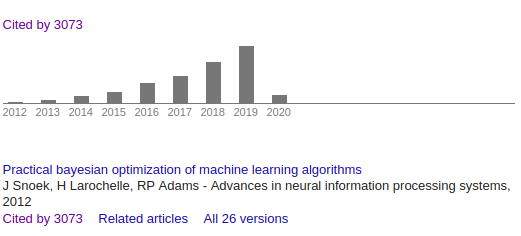
\includegraphics[width=.5\linewidth, keepaspectratio=true]{w07_hpo_grey_box/images/success_stories/spearmint_alt_stats.png}}
        \newline Google Scholar screenshot from 3rd March, 2020
    \end{center}
\end{itemize}
\end{frame}

%-----------------------------------------------------------------------
\begin{frame}[c]{Success Stories}
\framesubtitle{Hyperopt}
\begin{itemize}
    \item Hyperopt is another successful open source Bayesian optimization package.
    \item Implements the TPE algorithm and supports asynchronous parallel evaluations.
    \item Maintained since 2013.
    \item Available at \url{https://github.com/hyperopt/hyperopt}
\end{itemize}
\vspace{1cm}

\includegraphics[width=\linewidth, height=\textheight, keepaspectratio=true]{w07_hpo_grey_box/images/success_stories/hyperopt_git_stats.png}

\vspace{1cm}
\hspace{2cm}
\lit{\href{https://papers.nips.cc/paper/4443-algorithms-for-hyper-parameter-optimization.pdf}{Bergstra et al. 2011}}, \lit{\href{http://proceedings.mlr.press/v28/bergstra13.pdf}{Bergstra et al., 2013}}, \lit{\href{http://citeseerx.ist.psu.edu/viewdoc/download?doi=10.1.1.704.3494&rep=rep1&type=pdf}{Bergstra et al., 2013}}, \lit{\href{https://iopscience.iop.org/article/10.1088/1749-4699/8/1/014008/ampdf}{Bergstra et al., 2015}}

\end{frame}

%-----------------------------------------------------------------------
\begin{frame}[c]{Success Stories}
\framesubtitle{AlphaGo}
\begin{itemize}
    \item During the development of AlphaGo, its many hyperparameters
were tuned with Bayesian optimization multiple times.
    \item This automatic tuning process resulted in substantial improvements in playing strength. For example, prior to the match with Lee Sedol, we tuned the latest AlphaGo agent and this improved its win-rate from 50\% to 66.5\% in self-play games. This tuned version was deployed in the final match.
    \item Of course, since we tuned AlphaGo many times during its development cycle, the compounded contribution was even higher than this percentage.
\end{itemize}
\vspace{1cm}
\hspace{12cm}\lit{\href{https://arxiv.org/abs/1812.06855}{Chen et al.}}
\end{frame}

%-----------------------------------------------------------------------
\begin{frame}[c]{Success Stories}
\framesubtitle{Company usage}
\begin{itemize}
    \item SIGOPT: startup offering Bayesian optimization as a service.
    \item Facebook provides an open source Bayesian optimization package \lit{\href{https://botorch.org/}{BoTorch}}.
    \item Amazon provides an open source Bayesian optimization package \lit{\href{https://amzn.github.io/emukit/}{EmuKit}}.
    \item Uber tunes algorithms for \emph{Uber Pool}, \emph{UberX} and \emph{Uber Eats} \lit{\href{http://mcqmc2016.stanford.edu/Frazier-Peter.pdf}{source}}
    \item Many more, but less openly
\end{itemize}
\end{frame}

%-----------------------------------------------------------------------
\begin{frame}[c]{Success Stories}
\framesubtitle{Auto-WEKA}
\begin{itemize}
    \item Introduce Bayesian optimization for \emph{\textbf{C}ombined \textbf{A}lgorithm \textbf{S}election and \textbf{H}yperparameter optimization} problem (CASH problem).
    \begin{itemize}
        \item Each configuration $\conf$ comprises a choice of algorithm $A^{(j)} \in \mathcal{A}$
        \item Hyperparameters of $A^{(j)}$ are conditional on $A^{(j)}$ being selected
        \item $\argmin_{\conf} \frac{1}{k} \sum^k_{i=1} \loss(A^{(j)}_\lambda,\datasettrain,\datasetval)$
    \end{itemize}
    \item 768 hyperparameters, 4 leves of conditionality
    \item Based on WEKA and SMAC
\end{itemize}

\vspace{1cm}
\hspace{12cm}\lit{\href{https://link.springer.com/chapter/10.1007/978-3-030-05318-5_4}{Kotthoff et al. 2019}}

\end{frame}

%-----------------------------------------------------------------------